\chapter{Out-of-distribution Detection in High-dimensional Distributions} \label{ch-1}

\section{Motivation}

Modern machine learning has shown surprisingly unseen progress over the last decade and state-of-the-art performance for problems in many domains such as vision, natural language, time-series prediction, etc. has been improving constantly. A vital and sometimes overlooked assumption, however, is that the distribution at test time will closely follow that of the training time. In presence of distribution shifts, machine learning models can behave rather unpredictably. For example, figure \ref{fig:4-1} shows how a neural network can be over-confidently wrong in presence of distribution shift.

\begin{figure}[h]
    \centering
    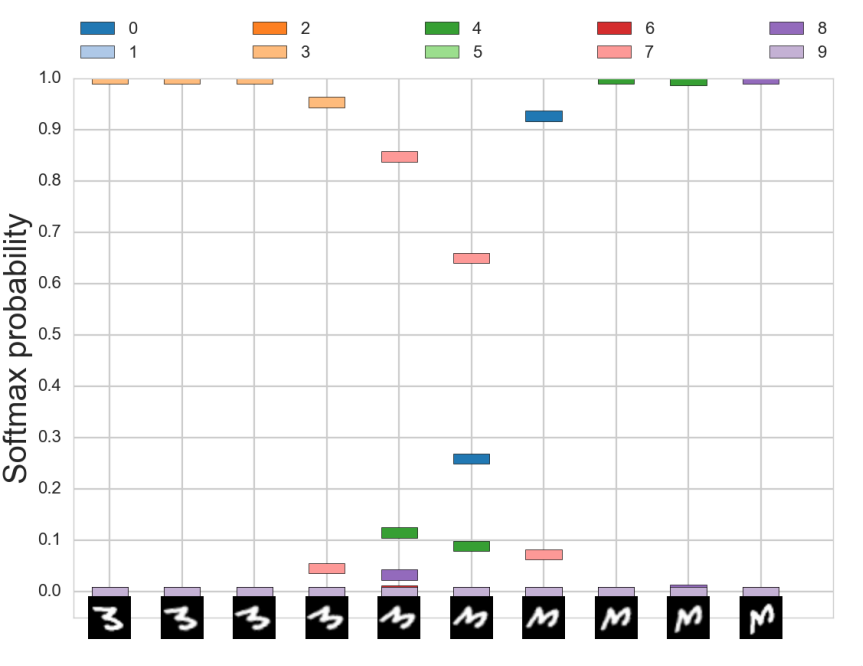
\includegraphics[width=0.5\textwidth]{figures/ch4/rotate3.png}
    \caption{Predictive distribution of LeNet for a continuously rotated version of a 3 from MNIST. Each color corresponds to a different class and the height of the bar denotes the probability assigned to that particular class by the network. Taken from \cite{louizos2017multiplicative}.}
    \label{fig:4-1}
\end{figure}

Therefore, carefully designed examples can easily fool discriminative models. Figure \ref{fig:4-2} shows an adversarial input designed to mislead a spam detection model. This can impose risks to any human in the loop application, especially in safety-critical domains. 

\begin{figure}[h]
    \centering
    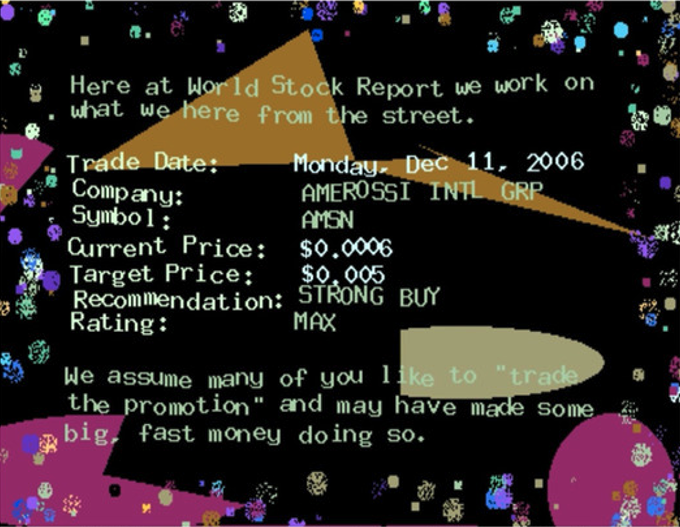
\includegraphics[width=0.4\textwidth]{figures/ch4/spam.png}
    \caption{Wild Patterns: Ten Years After the Rise of Adversarial Machine Learning \cite{biggio2018wild}.}
    \label{fig:4-2}
\end{figure}

In practice, ML pipelines rarely inspect incoming data for signs of distribution shift. Moreover, best practices for detecting shift in high-dimensional real-world data have not yet been established \cite{rabanser2019failing}. In addition to adversarial examples, out of distribution (OOD) detection is a basic building block of other tasks such as open-set recognition \cite{ren2019likelihood} and continual learning, where the systems are persistently observing unseen examples in run time.

\section{OOD Detection Using Generative Models}

One natural solution to OOD detection is using explicit likelihood models, as proposed by Bishop (1994). One would expect a generative model to return higher likelihood (probability density) for samples from training distributions compared to OOD samples. Therefore, thresholding the likelihood values is thought to be a simple and effective solution to OOD detection, as also proposed by Welling in AABI 2017 panel. However, Nalisnick, et al \cite{nalisnick2018deep} showed surprising counterexamples to challenge this intuition. This has been shown for a range of datasets and likelihood models. Ren et al. \cite{ren2019likelihood} also confirmed this observation on a genomic sequences dataset. 

\begin{figure}[h]
    \centering
    \vspace{-1em}
    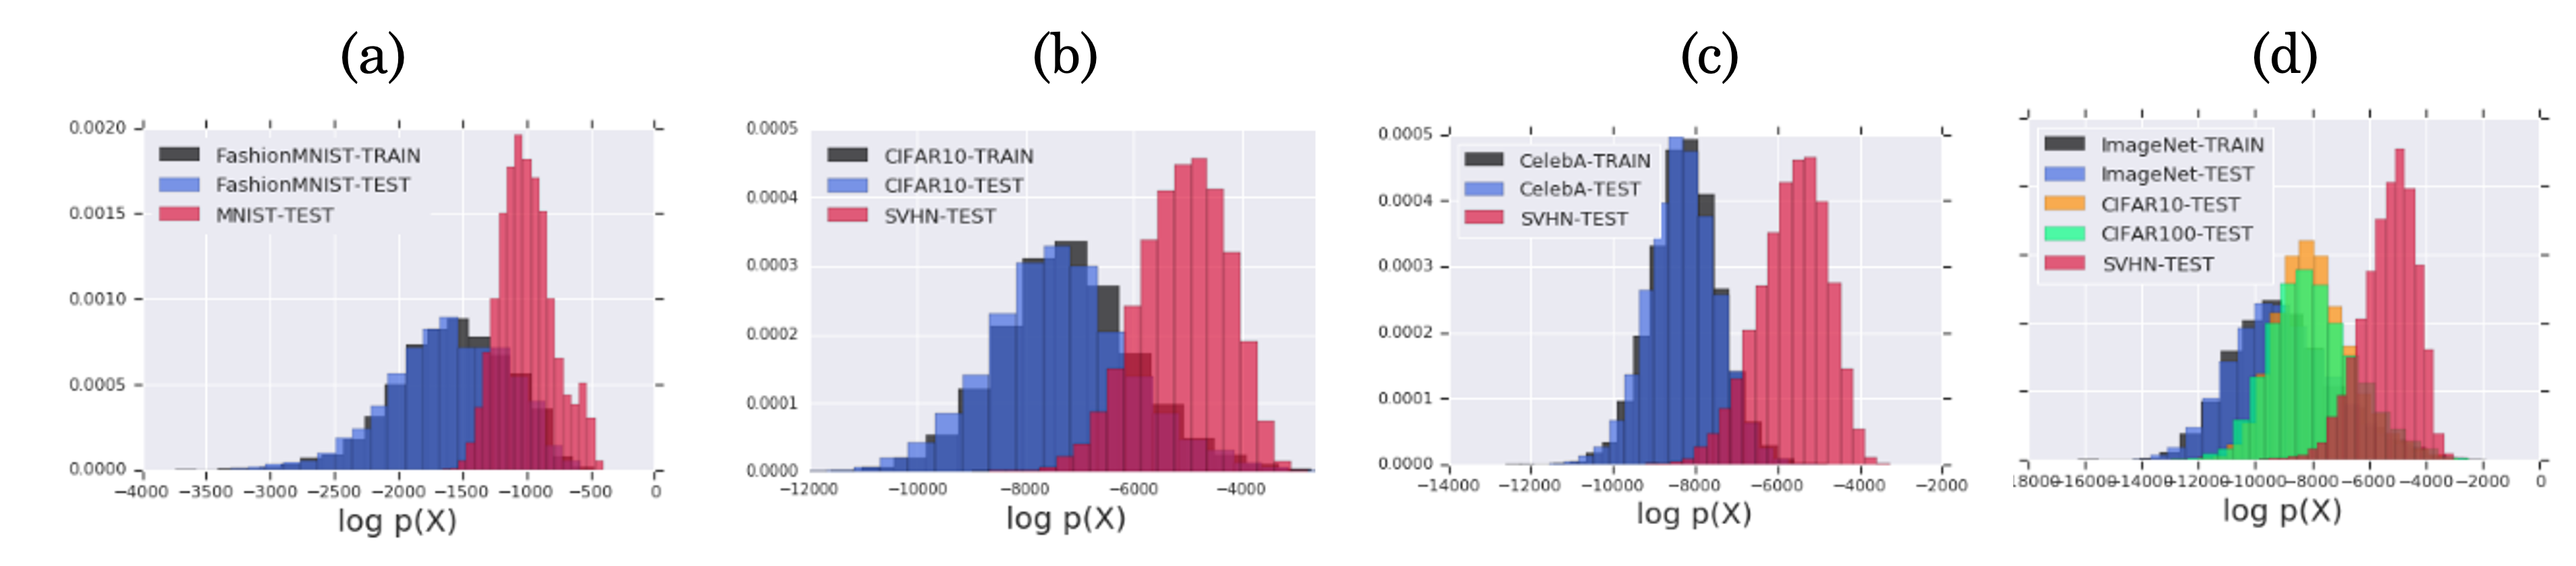
\includegraphics[width=\textwidth]{figures/ch4/nalisnic.png}
    \caption{Histogram of Glow log-likelihoods \cite{nalisnick2018deep}. (a) Train on FashionMNIST, Test on MNIST, (b) Train on CIFAR-10, Test on SVHN, (c) Train on CelebA, Test on SVHN, (d) Train on ImageNet, Test on CIFAR-10 / CIFAR-100 / SVHN.}
    \label{fig:4-3}
\end{figure}

At the time, this behavior was surprising enough to lead to questioning the correctness of our likelihood models. However, such phenomena can be naturally observed in basic settings. Consider a $d$-dimensional Gaussian distribution with independent coordinates, $X \sim \mathcal{N}(\bm{0}, I_d)$. Then, the distance of the samples to the mode of the distribution is chi distributed: $R = \sqrt{\sum_{i=1}^d X_i^2} \sim \chi(d)$. Examining the mean and variance of chi distribution for large values of $d$ reveals an interesting concentration property for samples of $X$. In high dimensional settings, $X$ takes values very close to the sphere of radius $\sqrt{d}$, and stays within constant distance from that sphere. This is also known as Gaussian Annulus Theorem \cite{vershynin2018high}.

\begin{remark}
The mean and variance of $R \sim \chi(d)$ for high degrees of freedom $d$:
\begin{align*}
    &\ex[R] = \sqrt{d} \left[1-\frac{1}{4d}+O\left(\frac{1}{d^2}\right)\right] \\
    &\var[R] = \frac{1}{2} + O\left(\frac{1}{d}\right)
\end{align*}
\end{remark}

Note that the mean of the high dimensional Gaussian has the highest likelihood value, however, it is not likely to observe any sample even in the neighborhood of the mean. This simple example shows the intuition that a PDF assigns higher likelihood to in-distribution samples than OOD samples is essentially invalid in high dimensions.

This separation of samples from high density regions can be explained by the tension between volume and density. Let us again consider our high dimensional Gaussian example and calculate probability density over concentric hyper-sphere shells around the origin. The infinitesimal volume of the hyper-sphere shell at radius $r$ is $\mathrm{d}V = S_{d}(r) \mathrm{d}r$, where $S_{d}(r)$ is the area of a $d$-dimensional hyper-sphere:
\begin{align}
    S_{d}(r) =  \frac{2 \pi^{d/2}}{\Gamma\left(\frac{d}{2}\right)} r^{d-1}
\end{align}

Therefore, the infinitesimal probability mass contained over such hyper-sphere shell is $ \mathrm{d}p = f(r) \mathrm{d}V = f(r) S_{d}(r) \mathrm{d}r$, where $f(r)$ is the Gaussian density at radius $r$: 
\begin{align}
    f(r) = (2\pi)^{-\frac{d}{2}}\exp(-\frac{r^2}{2})
\end{align}

Finally, the probability density over the sphere shell at radius $r$ can be calculated as:
\begin{align}
    g(r) &= \frac{\mathrm{d}p}{\mathrm{d}r} = f(r) S_{d}(r)  \nonumber \\
    &= \frac{1}{2^{\frac{d}{2}-1}\Gamma\left(\frac{d}{2}\right)} \exp(-\frac{r^2}{2}) \ r^{d-1} \label{eq:gr}
\end{align}

It is worth noting that Equation (\ref{eq:gr}) is the probability density function of $\chi(d)$ distribution. As we can see from Figure \ref{fig:4-4}, as we get further from the origin, density decreases while the volume of the shells increases at a higher rate. The tension of the two will cause the concentration of the samples in a region, commonly called the typical set.

\begin{figure}[h]
    \centering
    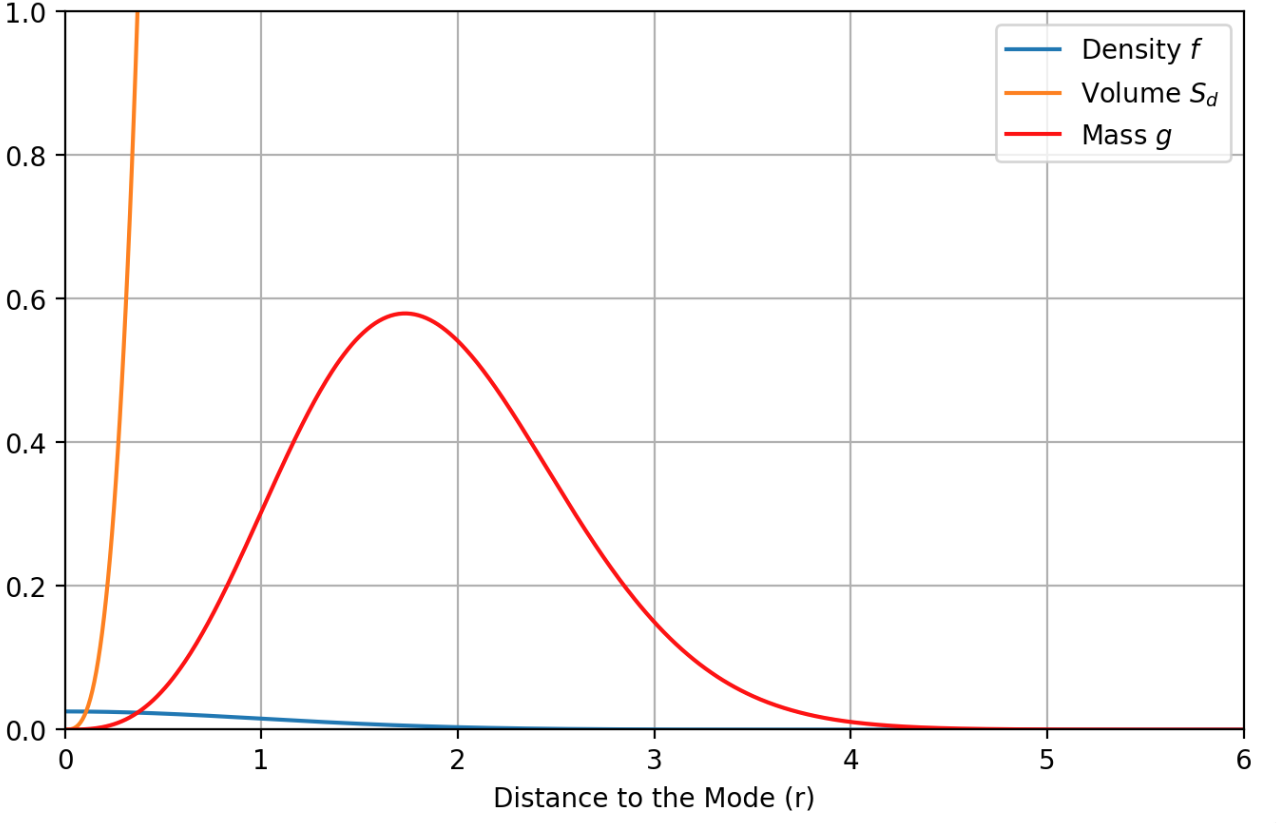
\includegraphics[width=0.6\textwidth]{figures/ch4/gaussian.png}
    \caption{Tension between density and volume causes concentration of samples.}
    \label{fig:4-4}
\end{figure}


\section{Related Works}
In the statistics literature, two-sample test and goodness-of-fit (GoF) tests are mature and well-studied subjects. In a two-sample test, given input data $\{x_i\}_1^N \sim p$ and $\{y_i\}_1^M \sim q$, the hypothesis test for $H_0: p=q$ vs. $H_A: p\neq q$ is considered. Similarly, in a goodness of fit setup, input samples  $\{x_i\}_1^N \sim p$ and a reference distribution $p_0$ are available for two hypotheses $H_0: p=p_0$ vs. $H_A: p\neq p\neq p_0$. Although for simple univariate distributions, such hypothesis testing is a mature science, best practices for two sample tests with high-dimensional (e.g. image) data remain an open question \cite{rabanser2019failing}. Examples of such tests include Maximum Mean Discrepancy (MMD), Kernelized Stein Discrepancy (KSD), and Kolmogorov–Smirnov test (KS). Many GoF tests rely on the CDF of the reference distributions. Two-sample methods require the original data to be stored and re-accessed, which may be a privacy and security limitation. For kernel-based multivariate two-sample tests like MMD, statistical power is known to decay badly with dimension \cite{ramdas2015decreasing}.

Likelihood ratio tests can be employed when a likelihood model of out of distribution data is available:
\begin{align*}
    p(x|ID) \lessgtr p(x|OOD) \frac{P(OOD)}{P(ID)},
\end{align*}

where $p(x|ID)$ is the likelihood model trained on the in-distribution data and $p(x|OOD)$ is the OOD model. Therefore, assuming a uniform OOD model is equivalent to the original intuition of thresholding the likelihood. \cite{meinke2019towards} trains a Gaussian Mixture Model using a dataset of 80 million tiny images to model OOD data. \cite{ren2019likelihood} uses noisy versions of the in-distribution dataset and calls it the "background" model to essentially build a likelihood model of OOD data. However, the main issue with this line of work is that $P(x|OOD)$ should model \textit{all} possible inputs that are not from the current distribution. This might be feasible for specific tasks or domains but cannot provide a general-purpose solution.

\section{Sample Complexity}
In pursuit of \textit{fixing} the likelihood models, Serra et al. \cite{serra2019input} provides an interesting observation connecting sample likelihood to its complexity. Figure \ref{fig:4-6} shows the surprising correlation between compression rates of images to their assigned likelihood.

\begin{figure}[h]
    \centering
    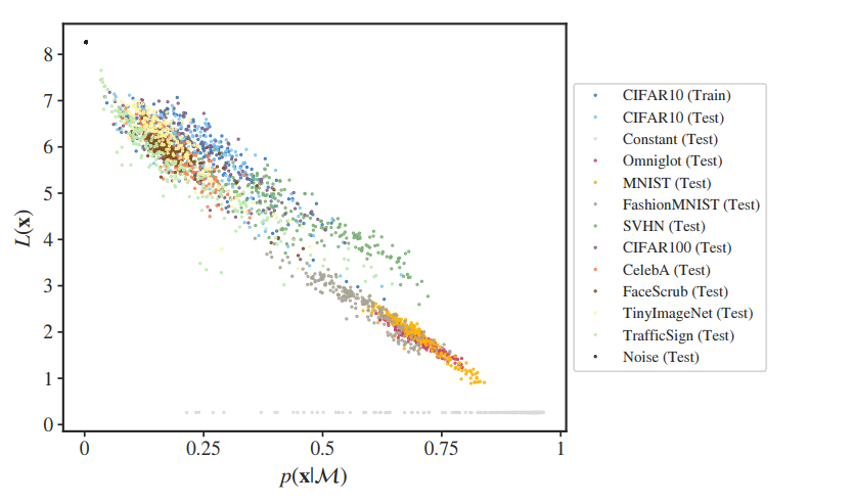
\includegraphics[width=0.8\textwidth]{figures/ch4/complexity.png}
    \caption{\cite{serra2019input} Normalized compressed lengths using a PNG compressor with respect to likelihoods of a PixelCNN++ model trained on CIFAR10.}
    \label{fig:4-6}
\end{figure}

In addition, similar results are shown for other likelihood models and compressors. As complexity seems to account for most of the variability in generative models’ likelihoods, they proposed to compensate for it when testing for possible OOD inputs. Therefore, given input $\bm{x}$ and assigned likelihood $l(\bm{x})$, the proposed test statistic is $S(\bm{x})=-l(\bm{x})-L(\bm{x})$, where $L(\bm{x})$ is the (normalized) compressed length of input $\bm{x}$ using a general lossless compressor. 

Here, we try to extend and explain this observation using the general notion of Kolmogorov complexity. But first, we show and analyze a similar observation for a simple i.i.d scenario. Consider random i.i.d sequence of $\bold{X} = X_1, \cdots, X_n$ where $X_i$'s are drawn according to distribution $Q$ on alphabet $\mathcal{X}$. Let us show the empirical distribution (type) of an observed sequence $\bm{x}$ by $P_\bm{x}$. It can be shown that the probability of observing $\bm{x}$ from type $P$ is $2^{-n \ KL(P, Q)}$ to first order in the exponent (\cite{elements}, Theorem 11.1.4). On the other hand, we have $Q^n(\bm{x})=2^{ -n( KL(P_{\bm{x}},Q) + H( P_{\bm{x}} ) )}$ (\cite{elements}, Theorem 11.1.2). This is the same observation as that of \cite{serra2019input}, where correcting the log-likelihood with a measure of sample complexity (in this case $H( P_{\bm{x}} )$) will result in $KL(P_{\bm{x}}, Q)$, which can act as a measure of OOD detection.

Correcting the log-likelihood with sample complexity can also be justified from a likelihood ratio test perspective. Considering Solomonoff’s universal probability as $P_\mathcal{U}(x)=2^{-K(x)}$ where $K(x)$ is the Kolmogorov complexity of data $x$, it is easy to see that using $\log P(x) - K(x) $ as a measure of OOD is equivalent to performing a likelihood ratio test for $P(x)$ vs. $P_\mathcal{U}(x)$, i.e. considering the universal probability as the OOD model. Such a choice for modeling the OOD is in line with the fact that an OOD likelihood model should encompass every possible input other than the distribution of interest. 

\section{Future Directions}

As briefly discussed in the previous section, the framework of algorithmic information theory provides a theoretical foundation to justify the use of sample complexity as a correction term for using likelihood as an OOD detection statistic. Further studying this connection can provide a grounding to support a practical solution to OOD detection.

Another interesting direction is the separation of the typical set and high-density regions. Such separation is discussed in \cite{betancourt2017conceptual}, where it is shown that efficient MCMC samplers like Hamiltonian Monte Carlo, can effectively identify and explore the typical set, given the likelihood information. Therefore, if MCMC samplers are capable of finding the typical set from the likelihood, one can frame the problem of OOD detection as \textit{verifying} if any given point belongs to the typical set. This connection between sampling and verification problems is another interesting direction.